\documentclass[12pt]{article}

% ── Codificación y lengua ─────────────────────────────────────────────────────
\usepackage[utf8]{inputenc}
\usepackage[spanish,es-nodecimaldot]{babel} % es-nodecimaldot mantiene el punto decimal
                                             % en fórmulas matemáticas (convención usada)

% ── Matemáticas y química ────────────────────────────────────────────────────
\usepackage{amsmath}
\usepackage[version=4]{mhchem}

% ── Gráficos y diseño de página ──────────────────────────────────────────────
\usepackage{graphicx}
\usepackage{geometry}
\geometry{margin=1in}

% ── Tablas ───────────────────────────────────────────────────────────────────
\usepackage{booktabs}
\usepackage{array}
\usepackage{longtable}

% ── Listas y columnas ────────────────────────────────────────────────────────
\usepackage{enumitem}
\usepackage{multicol}

% ── Referencias cruzadas con hipervínculos ───────────────────────────────────
\usepackage{hyperref}
\hypersetup{
    colorlinks = true,
    linkcolor  = black,
    citecolor  = black,
    urlcolor   = blue
}

% ── Regla horizontal compatible con LaTeX ────────────────────────────────────
\newcommand{\HRule}{\noindent\rule{\linewidth}{1pt}}

% ─────────────────────────────────────────────────────────────────────────────
\begin{document}

% ── ENCABEZADO ───────────────────────────────────────────────────────────────
\begin{figure}[h]
    \begin{minipage}{0.45\textwidth}
        \flushleft
        
\includegraphics[width=0.7\textwidth]{logo_escuela_quimica.png}
    \end{minipage}
    \hfill
    \begin{minipage}{0.45\textwidth}
        \flushright
        
\includegraphics[width=0.5\textwidth]{logo_yachay_tech.png}
    \end{minipage}
\end{figure}

\HRule
\vspace{0.5cm}

\begin{center}
    {\textbf{\large LABORATORIO DE QUÍMICA II}} \\[0.3cm]
    {\textbf{\large TEMA:}} \\[0.2cm]
    {Electroquímica y Celdas Galvánicas} \\[0.6cm]
\end{center}

\noindent
\begin{minipage}[t]{0.6\textwidth}
    \textbf{Entrega de informe:} 26/04/2026 \\[0.5cm]
    \textbf{Integrantes:}
    \begin{itemize}[leftmargin=1.5cm, label=\textbullet, itemsep=0.3cm]
        \item Baidal Saldarriaga Emily Marcela
        \item Vélez Reyes Daniel Steven
        \item Rojas Tuqueres Lisbeth Alexandra
        \item Nicolalde Haro Daniel Alexander
    \end{itemize}
\end{minipage}
\hfill
\begin{minipage}[t]{0.3\textwidth}
    \flushleft
    \textbf{Grupo:} 1 \\[0.3cm]
    \textbf{Paralelo:} PJ
\end{minipage}

\vspace{1cm}

% ── CUERPO DEL INFORME ───────────────────────────────────────────────────────

\section{Objetivos}

\begin{itemize}
    \item Comprender los principios fundamentales de las reacciones de
          óxido-reducción mediante el diseño y construcción de una celda
          galvánica para la conversión de energía química en energía eléctrica.
    \item Aplicar la ecuación de Nernst para predecir y verificar
          experimentalmente la fuerza electromotriz (FEM) bajo condiciones
          no estándar.
\end{itemize}

% ─────────────────────────────────────────────────────────────────────────────
\section{Fundamentación Teórica}

La electroquímica es la rama de la química que estudia la interconversión entre
la energía eléctrica y la energía química a través de procesos de transferencia
de electrones conocidos como reacciones de óxido-reducción (redox). Según Brown
en \textit{Química: La ciencia central}, estas reacciones son fundamentales en
la naturaleza y la tecnología, manifestándose en fenómenos que van desde la
corrosión de metales hasta el funcionamiento de dispositivos electrónicos
modernos. En una reacción redox, la sustancia que pierde electrones se oxida,
aumentando su estado de oxidación y actuando como agente reductor, mientras que
la sustancia que gana electrones se reduce, disminuyendo su estado de oxidación
y actuando como agente oxidante. Para aprovechar la energía liberada en una
reacción redox espontánea, es necesario separar físicamente las semirreacciones
de oxidación y reducción. Este diseño se denomina celda galvánica o voltáica,
donde cada componente se ubica en una semicelda distinta. Los electrones fluyen
desde el ánodo (donde ocurre la oxidación) hacia el cátodo (donde ocurre la
reducción) a través de un circuito externo. Para que el flujo de corriente sea
continuo, se emplea un puente salino o un tabique poroso que permite la
migración de iones entre las soluciones, manteniendo así la neutralidad
eléctrica de ambos compartimentos.

La fuerza impulsora detrás de este movimiento de electrones es la diferencia de
potencial eléctrico entre los electrodos, conocida como potencial de celda o
fuerza electromotriz (FEM). Este potencial depende directamente de la naturaleza
química de los materiales involucrados. En condiciones estándar (1~M de
concentración, 1~atm de presión y 25~°C), el potencial se mide frente al
electrodo estándar de hidrógeno. No obstante, en el entorno experimental de un
laboratorio, las condiciones suelen diferir de las ideales, lo que exige un
análisis más profundo de las variables que afectan el rendimiento energético de
la celda.

Finalmente, el comportamiento de una celda electroquímica en condiciones no
estándar se describe mediante la ecuación de Nernst. Esta relación matemática
establece que el potencial de la celda disminuye a medida que las
concentraciones de los reactivos se agotan o los productos aumentan, reflejando
la dependencia del voltaje respecto a la composición química del sistema. A
través de esta práctica, se busca validar experimentalmente estos principios
teóricos, comprendiendo cómo la variación en las concentraciones y la selección
de diferentes pares metálicos dictan la capacidad de una celda para generar
trabajo eléctrico útil.

% ─────────────────────────────────────────────────────────────────────────────
\section{Materiales y Métodos}

\subsection{Materiales y Reactivos}

\subsubsection*{Materiales}

\begin{multicols}{2}
\begin{itemize}[leftmargin=0.5cm, nosep]
    \item 2 Matraces Aforados de 10~ml.
    \item 2 Vasos de Precipitado de 25~ml.
    \item 1 Pipeta de 10~ml.
    \item 1 Hoja de papel de filtro.
    \item Papel de lija.
    \item 4 tubos de ensayo.
    \item 1 clavo.
    \item Polvo de hierro.
    \item Granos de zinc.
    \item Alambre de cobre.
    \item 2 Pinzas metálicas de cocodrilo.
    \item 1 Frasco lavador.
    \item 1 voltímetro.
    \item 2 Electrodos de cobre.
    \item 1 Electrodo de zinc.
\end{itemize}
\end{multicols}

\subsubsection*{Reactivos}

\begin{multicols}{2}
\begin{itemize}[leftmargin=0.5cm, nosep]
    \item Disolución de sulfato de cobre (\ce{CuSO4}, 0.2~M).
    \item Disolución de nitrato de zinc (\ce{Zn(NO3)2}, 0.2~M).
    \item Disolución de nitrato cúprico (\ce{Cu(NO3)2}, 0.1~M).
    \item Disolución de nitrato de potasio (\ce{KNO3}, 0.2~M).
    \item Ácido sulfúrico (\ce{H2SO4}, 1~M).
    \item Disolución de nitrato mercúrico (\ce{Hg(NO3)2}, 1~M).
    \item Agua destilada.
\end{itemize}
\end{multicols}

\newpage

\subsection{Métodos}

\begin{figure}[!htbp]
    \centering
    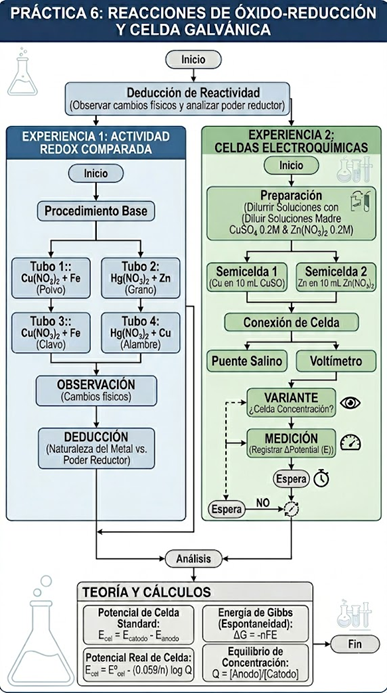
\includegraphics[width=0.65\textwidth]{Flujograma.png}
    \caption{Flujograma del procedimiento experimental.}
    \label{fig:flujograma}
\end{figure}

% ─────────────────────────────────────────────────────────────────────────────
\section{Resultados}

\subsection*{Experiencia 1: Reacciones de Óxido-Reducción}

Se evaluó la reactividad de distintos metales en contacto con soluciones
electrolíticas para observar procesos de transferencia de electrones de manera
directa. Para cada caso, se depositó el metal sólido en un tubo de ensayo con
la solución correspondiente y se registraron los cambios físicos inmediatos.

\begin{table}[!htbp]
\centering
\renewcommand{\arraystretch}{2}
\begin{tabular}{|>{\centering\arraybackslash}m{6.8cm}
                |>{\centering\arraybackslash}m{3cm}
                |>{\centering\arraybackslash}m{5.5cm}|}
\hline
\textbf{Reacciones} &
\textbf{Estados de oxidación} &
\textbf{Semirreacciones y observaciones} \\ \hline

\ce{H2SO4 + Fe -> FeSO4 + H2} &
$H{:}\ +1 \to 0$ \newline
$Fe{:}\ 0 \to +2$ \newline
$S{:}\ +6$ \newline
$O{:}\ -2$ &
\textit{Oxi:} \ce{Fe^0 -> Fe^{2+} + 2e-} \newline
\textit{Red:} \ce{2H+ + 2e- -> H2} \newline
\textbf{Observaciones:} Se observó oxidación y formación de burbujas gaseosas.
\\ \hline

\ce{CuSO4 + Zn -> ZnSO4 + Cu} &
$Zn{:}\ 0 \to +2$ \newline
$Cu{:}\ +2 \to 0$ &
\textit{Oxi:} \ce{Zn^0 -> Zn^{2+} + 2e-} \newline
\textit{Red:} \ce{Cu^{2+} + 2e- -> Cu^0} \newline
\textbf{Observaciones:} Cambio de coloración a un tono más claro.
\\ \hline

\ce{Hg(NO3)2 + Zn -> Zn(NO3)2 + Hg} &
$Zn{:}\ 0 \to +2$ \newline
$Hg{:}\ +2 \to 0$ &
\textit{Oxi:} \ce{Zn^0 -> Zn^{2+} + 2e-} \newline
\textit{Red:} \ce{Hg^{2+} + 2e- -> Hg^0} \newline
\textbf{Observaciones:} La pepita de zinc se disolvió progresivamente hasta desintegrarse.
\\ \hline

\ce{Hg(NO3)2 + Cu -> Cu(NO3)2 + Hg} &
$Cu{:}\ 0 \to +2$ \newline
$Hg{:}\ +2 \to 0$ &
\textit{Oxi:} \ce{Cu^0 -> Cu^{2+} + 2e-} \newline
\textit{Red:} \ce{Hg^{2+} + 2e- -> Hg^0} \newline
\textbf{Observaciones:} Cambio de coloración en el alambre de cobre.
\\ \hline
\end{tabular}
\caption{Resultados de reacciones redox y observaciones experimentales.}
\label{tab:redox}
\end{table}

Según los principios descritos por Brown~\cite{brown2014}, cuando un metal se
introduce en una solución electrolítica que contiene iones de un metal menos
activo, ocurre una transferencia espontánea de electrones. En este fenómeno,
el metal sólido actúa como agente reductor (se oxida), mientras que los
cationes en solución funcionan como agente oxidante (se reducen). Los
resultados se contrastan con la serie de actividad de los metales, la cual
predice la viabilidad de estas reacciones basándose en la facilidad con la que
un elemento cede electrones para formar cationes.

\subsection*{Experiencia 2: Celdas Galvánicas y Ecuación de Nernst}

Se construyeron celdas electroquímicas conectando dos semiceldas mediante un
puente salino impregnado con solución salina. Se utilizó un multímetro digital
para medir la diferencia de potencial (voltaje) entre los electrodos de zinc y
cobre, variando las concentraciones de los electrolitos para analizar el
comportamiento del sistema frente a condiciones no estándar.

\begin{table}[!htbp]
\centering
\renewcommand{\arraystretch}{1.5}
\begin{tabular}{|c
                |>{\centering\arraybackslash}m{3cm}
                |>{\centering\arraybackslash}m{3cm}
                |c|c|}
\hline
\textbf{Celda} &
\textbf{Concentración de \ce{Zn(NO3)2}} &
\textbf{Concentración de \ce{CuSO4}} &
\textbf{Voltaje exp. (V)} &
\textbf{Voltaje teo. (V)} \\ \hline
1 & 0.1~M  & 0.1~M  & 0.917 & 1.100 \\ \hline
2 & 0.05~M & 0.05~M & 0.905 & 1.100 \\ \hline
3 & 0.1~M  & 0.05~M & 0.904 & 1.091 \\ \hline
4 & 0.05~M & 0.1~M  & 0.912 & 1.109 \\ \hline
\end{tabular}
\caption{Resultados de medición de voltaje en celdas galvánicas.}
\label{tab:celdas}
\end{table}

Con los resultados de la Tabla~\ref{tab:celdas} se formulan las siguientes
observaciones:

\begin{itemize}
    \item \textbf{Dependencia de $Q$:} En la Celda~3, al ser
          $[\text{Zn}^{2+}] > [\text{Cu}^{2+}]$, el valor de $Q$ es mayor a
          1, lo que según la ecuación de Nernst debe disminuir el voltaje de
          la celda (como se observa al comparar 0.917~V vs.\ 0.904~V). En la
          Celda~4 ocurre lo contrario: al aumentar la concentración del
          reactivo \ce{Cu^{2+}}, el sistema favorece la formación de
          productos, aumentando la FEM.

    \item \textbf{Desviación del valor estándar:} Los valores experimentales
          se mantuvieron consistentemente cerca de los 0.91~V, alejándose del
          valor teórico de 1.10~V. Esta discrepancia puede atribuirse a la
          resistencia interna del multímetro, a la formación de capas de
          óxido pasivantes en los electrodos y a la pureza de los reactivos.

    \item \textbf{Comparación de Celdas~1 y 2:} Teóricamente, si $Q = 1$ en
          ambas, el voltaje debería ser idéntico. La pequeña variación
          observada (0.917~V vs.\ 0.905~V) ilustra que, en condiciones
          reales, la concentración absoluta también influye levemente en la
          eficiencia de la transferencia de carga.
\end{itemize}

% ─────────────────────────────────────────────────────────────────────────────
\section{Discusión}

En la primera experiencia, se validó la serie de actividades de los metales
mediante la observación de transferencias directas de electrones en tubos de
ensayo. La presencia de burbujas en la reacción con \ce{H2SO4} y los cambios
de coloración al introducir hierro y zinc en las soluciones de cobre y mercurio
confirman que estos metales actuaron como agentes reductores espontáneos. Estos
fenómenos demuestran que el hierro y el zinc poseen mayor facilidad para ceder
electrones en comparación con los cationes en solución, permitiendo que la
reacción ocurra sin energía externa.

Por otro lado, en la Experiencia~2 la separación física de las semirreacciones
permitió canalizar el flujo de electrones a través de un circuito externo,
generando una diferencia de potencial medible. A pesar de que los voltajes
experimentales se mantuvieron estables alrededor de 0.91~V, existió una
desviación significativa respecto al valor teórico de 1.10~V.

Esta variabilidad se atribuye a la resistencia interna del sistema y a la
posible formación de capas de óxido pasivantes en los electrodos, lo que
justifica el uso de lija para exponer la superficie activa. Así mismo, el
puente salino introduce una resistencia adicional que disminuye la FEM real
captada por el voltímetro.

Por último, el análisis de las variaciones en la concentración de los
electrolitos permitió verificar la sensibilidad del potencial de celda respecto
al cociente de reacción ($Q$). En la Celda~3, donde la concentración del
producto \ce{Zn^{2+}} fue superior a la del reactivo \ce{Cu^{2+}}, se registró
una disminución en el voltaje (0.904~V), coherente con la ecuación de Nernst,
ya que un valor de $Q > 1$ reduce el potencial total del sistema. Por el
contrario, al aumentar la concentración de reactivos en la Celda~4, la FEM
mostró una tendencia al aumento. Estas variaciones subrayan que la capacidad
de una celda para generar trabajo eléctrico depende directamente de la
disponibilidad de iones y se degrada conforme el sistema se aproxima al
equilibrio químico, donde $Q = K$ y el potencial llega a 0~V.

% ─────────────────────────────────────────────────────────────────────────────
\section{Conclusiones}

\begin{itemize}
    \item Se comprendieron los principios de las reacciones redox al construir
          una celda galvánica funcional, donde la separación física de las
          semirreacciones permitió que la transferencia espontánea de
          electrones se manifestara como energía eléctrica aprovechable. La
          observación de cambios físicos en los electrodos y la medición de
          voltaje confirmaron que la energía liberada en la reacción química
          puede transformarse en trabajo eléctrico mediante un flujo ordenado
          de electrones desde el ánodo hacia el cátodo.

    \item La aplicación de la ecuación de Nernst verificó que el potencial de
          la celda es altamente sensible a las variaciones en las
          concentraciones de los electrolitos. Los resultados demostraron que
          cuando el cociente de reacción ($Q$) aumenta, el potencial de la
          celda disminuye, lo que permite predecir y comprobar la tendencia
          del sistema hacia el equilibrio químico, donde el potencial
          eléctrico finalmente se anula.
\end{itemize}

% ─────────────────────────────────────────────────────────────────────────────
\section{Cuestiones}

\begin{enumerate}[label=\textbf{P\arabic*.}, leftmargin=1.2cm]

    \item \textbf{¿Qué factores pueden influir sobre el voltaje obtenido en la
          experimentación?}

    La fuerza electromotriz (FEM) de una celda galvánica no es un valor
    estático; su magnitud experimental está condicionada por diversos factores
    termodinámicos y cinéticos:

    \begin{itemize}[leftmargin=1cm]
        \item \textbf{Naturaleza de los metales:} La diferencia entre los
              potenciales estándar de reducción de los dos electrodos es el
              factor principal.
        \item \textbf{Concentración de los electrolitos:} Como indica la
              ecuación de Nernst, el potencial varía según la concentración
              de los iones en solución.
        \item \textbf{Temperatura:} La energía cinética de las partículas
              afecta la movilidad iónica y el potencial termodinámico.
        \item \textbf{Resistencia interna:} La pureza de los metales y la
              eficiencia del puente salino pueden reducir el voltaje medido
              respecto al teórico.
    \end{itemize}

    \item \textbf{Habitualmente cuando realizamos los experimentos en
          laboratorio se obtiene un mejor resultado cuando usamos papel de
          lija para limpiar los metales. ¿Por qué?}

    Los metales expuestos al aire forman una capa de óxido o impurezas en su
    superficie debido a la corrosión natural~\cite{brown2014}. Esta capa actúa
    como aislante, impidiendo el contacto directo entre el metal puro y la
    solución electrolítica, lo que aumenta la resistencia y dificulta la
    transferencia de electrones. Al lijar el metal se elimina esa barrera y se
    expone la superficie activa del electrodo, optimizando la reacción.

    \item \textbf{Cuando cambiamos de concentración podemos usar la ecuación
          de Nernst. ¿Esta ecuación se puede usar con cualquier concentración
          de iones?}

    Teóricamente, la ecuación de Nernst es aplicable a cualquier
    concentración. Sin embargo, en la práctica existen limitaciones:

    \begin{itemize}[leftmargin=1cm]
        \item \textbf{Disoluciones muy concentradas:} Las interacciones
              electrostáticas entre iones son tan fuertes que la
              ``concentración efectiva'' (actividad) es menor que la
              concentración molar.
        \item \textbf{Disoluciones extremadamente diluidas:} El potencial
              se vuelve inestable y difícil de medir con precisión. Para
              cálculos de laboratorio estándar se asume que la molaridad es
              igual a la actividad.
    \end{itemize}

    \item \textbf{¿Por qué una celda galvánica puede perder su actividad con
          el tiempo?}

    Una pila ``muere'' principalmente por dos razones:

    \begin{itemize}[leftmargin=1cm]
        \item \textbf{Agotamiento de reactivos:} A medida que la reacción
              progresa, la concentración de los reactivos disminuye y la de
              los productos aumenta hasta que el sistema alcanza el
              equilibrio químico ($Q = K$). En el equilibrio,
              $E_{\text{celda}} = 0$~V.
        \item \textbf{Polarización y degradación:} El puente salino puede
              secarse o saturarse, impidiendo la neutralidad eléctrica, o los
              electrodos pueden cubrirse de subproductos que detienen la
              transferencia electrónica.
    \end{itemize}

    \item \textbf{¿Es posible hacer una celda galvánica considerando el aire
          como una semicelda?}

    Sí, es posible. Un ejemplo común son las celdas de combustible de
    hidrógeno-oxígeno o las baterías de zinc-aire. En estos sistemas, el
    oxígeno del aire actúa como agente oxidante en el cátodo:
    \[
        O_2\text{(g)} + 2\,H_2O\text{(l)} + 4\,e^- \;\to\; 4\,OH^-\text{(ac)}
    \]
    El aire es una fuente abundante de oxígeno, lo que permite diseñar celdas
    más ligeras, ya que no necesitan cargar con el oxidante sino que lo toman
    del ambiente.

\end{enumerate}

% ─────────────────────────────────────────────────────────────────────────────
\section{Sección Actúa}

\begin{enumerate}[label=\textbf{\alph*)}, leftmargin=1.2cm]

    \item \textbf{En la guía de la práctica existe una descripción detallada
          de la ecuación de Nernst. Comente si los resultados experimentales
          son adecuados a la teoría de Nernst y explique cómo deberían ser
          los voltajes teóricos.}

    Cálculo de voltajes teóricos con la ecuación de Nernst ($T = 298$~K) para
    la celda:
    \[
        \text{Zn(s)} \mid \text{Zn}^{2+}\text{(ac)}
        \parallel
        \text{Cu}^{2+}\text{(ac)} \mid \text{Cu(s)}
    \]
    \[
        E^\circ = E^\circ\!\left(\frac{\text{Cu}^{2+}}{\text{Cu}}\right)
                - E^\circ\!\left(\frac{\text{Zn}^{2+}}{\text{Zn}}\right)
                = 0.34\ \text{V} - (-0.76\ \text{V}) = 1.10\ \text{V}
        \qquad n = 2
    \]
    \[
        E = E^\circ - \frac{0.059\ \text{V}}{n}\,\log Q,
        \qquad
        Q = \frac{[\text{Zn}^{2+}]}{[\text{Cu}^{2+}]}
    \]

    \begin{table}[h!]
    \centering
    \renewcommand{\arraystretch}{1.5}
    \begin{tabular}{|c|c|c|c|c|c|c|}
    \hline
    \textbf{Celda} &
    \textbf{$[\text{Zn}^{2+}]$ (M)} &
    \textbf{$[\text{Cu}^{2+}]$ (M)} &
    \textbf{$Q$} &
    \textbf{$\log Q$} &
    \textbf{$E_\text{teo}$ (V)} &
    \textbf{$E_\text{exp}$ (V)} \\ \hline
    1 & 0.10 & 0.10 & 1.00 &  0.000 & 1.100 & 0.917 \\ \hline
    2 & 0.05 & 0.05 & 1.00 &  0.000 & 1.100 & 0.905 \\ \hline
    3 & 0.10 & 0.05 & 2.00 &  0.301 & 1.091 & 0.904 \\ \hline
    4 & 0.05 & 0.10 & 0.50 & -0.301 & 1.109 & 0.912 \\ \hline
    \end{tabular}
    \caption{Comparación de voltajes teóricos y experimentales mediante la
             ecuación de Nernst.}
    \label{tab:nernst}
    \end{table}

    La teoría predice que las Celdas~1 y 2 deben tener el mismo voltaje
    (1.100~V, pues $Q = 1$), que la Celda~3 sea ligeramente menor que la~1 y
    que la Celda~4 sea ligeramente mayor. Experimentalmente se observa la
    tendencia cualitativa correcta, aunque el valor absoluto se aleja del
    teórico. Los resultados no son correctos en términos absolutos, pero sí
    validan cualitativamente la ecuación de Nernst al mostrar la dependencia
    del voltaje con la concentración.

    % ─────────────────────────────────────────────────────────────────────────
    \item \textbf{Comente de manera simple (aprox.\ 100~palabras por caso) de
          qué manera se relaciona la electroquímica con las baterías de los
          autos eléctricos, los electrocardiogramas, la respiración en los
          animales y las celdas de combustible.}

    \noindent\textbf{Baterías de autos eléctricos}

    Los vehículos eléctricos utilizan baterías recargables de ion-litio o de
    níquel-metal. En estas celdas electroquímicas, la energía química
    almacenada en los electrodos se convierte en electricidad durante la
    descarga y se repone durante la carga. El ánodo de grafito libera
    electrones que viajan por un circuito externo hacia el cátodo de óxido
    metálico, mientras los iones $\text{Li}^+$ migran a través del
    electrolito. La eficiencia, autonomía y seguridad dependen de los
    materiales y del diseño electroquímico~\cite{rodriguez,stanford}.

    \vspace{0.4cm}
    \noindent\textbf{Electrocardiogramas}

    El corazón late gracias a diferencias de potencial eléctrico generadas por
    flujos iónicos ($\text{Na}^+$, $\text{K}^+$, $\text{Ca}^{2+}$) a través
    de membranas celulares. El electrocardiograma mide estos potenciales en la
    superficie corporal mediante electrodos de plata/cloruro de plata. Cada
    complejo P-QRS-T refleja despolarizaciones y repolarizaciones auriculares y
    ventriculares. La ecuación de Nernst explica el potencial de reposo
    ($-70$~mV) y los cambios durante el latido~\cite{khan,unam}.

    \vspace{0.4cm}
    \noindent\textbf{Respiración y transporte de oxígeno por hemoglobina}

    La hemoglobina contiene cuatro grupos hemo, cada uno con un átomo de
    hierro en estado $\text{Fe}^{2+}$ que se une reversiblemente al
    $\text{O}_2$. Este proceso implica una leve transferencia de densidad
    electrónica, es decir, una reacción redox parcial. Al oxidarse a
    $\text{Fe}^{3+}$ (metahemoglobina), pierde capacidad de transportar
    oxígeno; el citocromo $b_5$ reductasa la regenera. Así, la respiración
    celular depende de reacciones electroquímicas que permiten el transporte
    eficiente de $\text{O}_2$ desde los pulmones a los
    tejidos~\cite{sepulveda2020}.

    \vspace{0.4cm}
    \noindent\textbf{Celdas de combustible}

    Las celdas de combustible convierten directamente energía química de
    $\text{H}_2$ y $\text{O}_2$ en electricidad sin combustión. En la celda de
    membrana de intercambio protónico (PEM), el $\text{H}_2$ se oxida en el
    ánodo liberando electrones que viajan por un circuito externo, mientras los
    protones atraviesan la membrana y se combinan con $\text{O}_2$ en el cátodo
    para formar agua. Son eficientes, limpias y se usan en vehículos de
    hidrógeno y aplicaciones estacionarias~\cite{rozo2007,huazhong}.

    % ─────────────────────────────────────────────────────────────────────────
    \item \textbf{Traduzca y transcriba tres problemas resueltos del capítulo
          ``Electrochemistry'' del libro \textit{Chemistry~--~The Central
          Science}~\cite{brown2014}.}

    \vspace{0.4cm}
    \noindent\textbf{Ejercicio~19.9: Determinar la espontaneidad}

    Usando los potenciales estándar de reducción (Tabla~19.1), determine si
    las siguientes reacciones son espontáneas bajo condiciones estándar.

    \begin{enumerate}[label=(\alph*)]
        \item $\text{Cu(s)} + 2\,\text{H}^+\text{(ac)}
               \rightarrow \text{Cu}^{2+}\text{(ac)} + \text{H}_2\text{(g)}$
        \item $\text{Cl}_2\text{(g)} + 2\,\text{I}^-\text{(ac)}
               \rightarrow 2\,\text{Cl}^-\text{(ac)} + \text{I}_2\text{(s)}$
    \end{enumerate}

    \textbf{Solución:} Para determinar si una reacción redox es espontánea
    bajo condiciones estándar, se escriben sus semirreacciones y se calcula
    $E^\circ$. La reacción es espontánea si $E^\circ > 0$.

    \textit{Desarrollo (a):}
    \begin{align*}
        \text{Reducción:} &\quad
          2\,\text{H}^+\text{(ac)} + 2\,e^- \to \text{H}_2\text{(g)}
          & E^\circ_\text{red} &= 0\ \text{V} \\
        \text{Oxidación:} &\quad
          \text{Cu(s)} \to \text{Cu}^{2+}\text{(ac)} + 2\,e^-
          & E^\circ_\text{red} &= +0.34\ \text{V}
    \end{align*}
    \[
        E^\circ = 0\ \text{V} - 0.34\ \text{V} = -0.34\ \text{V}
        \quad \Rightarrow \quad \text{No espontánea.}
    \]

    \textit{Desarrollo (b):}
    \begin{align*}
        \text{Reducción:} &\quad
          \text{Cl}_2\text{(g)} + 2\,e^- \to 2\,\text{Cl}^-\text{(ac)}
          & E^\circ_\text{red} &= +1.36\ \text{V} \\
        \text{Oxidación:} &\quad
          2\,\text{I}^-\text{(ac)} \to \text{I}_2\text{(s)} + 2\,e^-
          & E^\circ_\text{red} &= +0.54\ \text{V}
    \end{align*}
    \[
        E^\circ = 1.36\ \text{V} - 0.54\ \text{V} = +0.82\ \text{V}
        \quad \Rightarrow \quad \text{Espontánea.}
    \]

    \vspace{0.6cm}
    \noindent\textbf{Ejercicio~19.6: Cálculo de $E^\circ_\text{celda}$ a
    partir de $E^\circ_\text{red}$}

    \textbf{Solución:} Se identifican las semirreacciones del cátodo y del
    ánodo, y se aplica:
    \[
        E^\circ_\text{celda} = E^\circ_\text{red}\text{(cátodo)}
                             - E^\circ_\text{red}\text{(ánodo)}
    \]

    \begin{align*}
        \text{Cátodo:} &\quad
          \text{Cr}_2\text{O}_7^{2-}\text{(ac)}
          + 14\,\text{H}^+\text{(ac)} + 6\,e^-
          \to 2\,\text{Cr}^{3+}\text{(ac)} + 7\,\text{H}_2\text{O(l)} \\
        \text{Ánodo:}  &\quad
          6\,\text{I}^-\text{(ac)}
          \to 3\,\text{I}_2\text{(s)} + 6\,e^-
    \end{align*}
    \[
        E^\circ_\text{celda} = 1.33\ \text{V} - 0.54\ \text{V} = 0.79\ \text{V}
        \quad \Rightarrow \quad \text{Celda espontánea.}
    \]
    El valor de $E^\circ$ no se multiplica al escalar la semirreacción, ya
    que es una propiedad intensiva.

    \vspace{0.6cm}
    \noindent\textbf{Ejercicio~19.13: Determinar el pH usando una celda de
    concentración}

    \textbf{Solución:} Se usa la ecuación de Nernst con
    $E^\circ_\text{celda} = 0$ (celda de concentración) y $n = 2$:
    \[
        E = -\frac{0.0256\ \text{V}}{n}\,\ln Q
    \]
    \[
        0.211\ \text{V}
        = -\frac{0.0256\ \text{V}}{2}\,\ln Q
        \implies
        \ln Q = \frac{-0.211}{0.0128} = -16.48
        \implies
        Q = e^{-16.48} = 6.9 \times 10^{-8}
    \]
    \[
        [\text{H}^+] = 6.9 \times 10^{-8}\ \text{M}
        \implies
        \text{pH} = -\log[\text{H}^+] \approx 7.16
    \]

    % ─────────────────────────────────────────────────────────────────────────
    \item \textbf{¿Por qué es importante la electroquímica?}

    La electroquímica es fundamental porque explica y permite la conversión
    entre energía química y eléctrica. Sin ella, no existirían las baterías que
    alimentan teléfonos, computadoras y autos eléctricos, ni las celdas de
    combustible que prometen un futuro energético limpio. En medicina, los
    electrocardiogramas, marcapasos y sensores de glucosa dependen de
    principios electroquímicos.

    Además, procesos industriales como la producción de aluminio, cloro e
    hidrógeno mediante electrólisis, así como la prevención de la corrosión,
    se basan en esta disciplina. Incluso la vida misma es electroquímica: la
    respiración, el transporte de oxígeno por hemoglobina y los impulsos
    nerviosos involucran transferencias controladas de electrones e iones.
    Comprender la electroquímica es, por tanto, comprender cómo funciona el
    mundo desde lo más pequeño (células) hasta lo más grande (redes
    energéticas).

\end{enumerate}

% ─────────────────────────────────────────────────────────────────────────────
\section{Ficha Bibliográfica}

\renewcommand{\arraystretch}{1.4}
\begin{longtable}{|p{4.5cm}|p{11.5cm}|}
\hline
\textbf{Concepto} & \textbf{Descripción} \\ \hline
\endfirsthead
\hline
\textbf{Concepto} & \textbf{Descripción} \\ \hline
\endhead
\hline
\endfoot
\hline
\endlastfoot

Nombre de la investigación en español &
Construcción y operación de una celda de combustible microbiana con análisis
de bacterias electroactivas \\ \hline

Autores y afiliación &
Kaline Araújo Soares. Universidade Federal do Ceará (UFC), Departamento de
Engenharia Mecânica. Orientadora: Prof.\ Dra.\ Fernanda Leite Lobo. \\ \hline

Revista y fecha de publicación &
Tesis de Maestría, defendida el 16 de febrero de 2024. \\ \hline

Traducción del resumen &
Las celdas de combustible microbianas (MFC) son tecnologías que utilizan
microorganismos para convertir sustratos orgánicos en energía eléctrica y
tratar aguas residuales. Se construyeron y operaron dos MFC con consorcios
microbianos mixtos. La caracterización electroquímica incluyó voltaje de
circuito abierto, voltamperometría de barrido lineal (LSV) y demanda química
de oxígeno (DQO). El análisis del gen $16\text{S rRNA}$ identificó como
géneros predominantes \textit{Camamonas}, \textit{Serratia},
\textit{Paraclostridium}, \textit{Bacillus} y \textit{Clostridium}. MFC1
alcanzó $600 \pm 0.2\ \text{mW/m}^2$ y MFC2 registró
$350 \pm 0.5\ \text{mW/m}^2$. Se concluye que los cultivos mixtos son
efectivos y robustos para la generación de bioelectricidad. \\ \hline

Resultados más relevantes &
\begin{itemize}[leftmargin=0.4cm, nosep]
    \item MFC1 alcanzó $600 \pm 0.2\ \text{mW/m}^2$; MFC2 logró
          $350 \pm 0.5\ \text{mW/m}^2$.
    \item Voltaje asociado de $550\ \text{mV}$ en las celdas operadas.
    \item Géneros predominantes en el biofilm anódico: \textit{Camamonas},
          \textit{Serratia}, \textit{Paraclostridium}, \textit{Bacillus} y
          \textit{Clostridium}.
    \item Remoción de DQO entre 55\,\% y 85\,\% según la carga orgánica.
\end{itemize} \\ \hline

Métodos de análisis utilizados &
\begin{itemize}[leftmargin=0.4cm, nosep]
    \item Inoculación con consorcio microbiano mixto de lodo.
    \item Voltamperometría de barrido lineal (LSV).
    \item Determinación de DQO (método APHA).
    \item Secuenciamiento del gen $16\text{S rRNA}$.
\end{itemize} \\ \hline

Conclusiones &
Es posible construir MFC con cultivos mixtos, logrando generación significativa
de energía ($600\ \text{mW/m}^2$) y remoción de materia orgánica. Los géneros
dominantes difieren de los clásicos \textit{Geobacter} y \textit{Shewanella},
lo que amplía el conocimiento sobre bacterias electroactivas. \\ \hline

Bibliografía del artículo (APA) &
Soares, K. A. (2024). \textit{Construção e operação de uma célula combustível
microbiana com análise de bactérias eletroativas} [Dissertação de mestrado,
Universidade Federal do Ceará]. Repositório Institucional UFC. \\ \hline

Cinco investigaciones relacionadas (APA) &
\begin{enumerate}[leftmargin=0.4cm, nosep]
    \item Logan, B. E., \& Rabaey, K. (2012). Conversion of wastes into
          bioelectricity and chemicals by using microbial electrochemical
          technologies. \textit{Science}, \textit{337}(6095), 686--690.
          \url{https://doi.org/10.1126/science.1217412}
    \item Lovley, D. R. (2006). Bug juice: harvesting electricity with
          microorganisms. \textit{Nature Reviews Microbiology},
          \textit{4}(7), 497--508.
          \url{https://doi.org/10.1038/nrmicro1442}
    \item Santoro, C., Arbizzani, C., Erable, B., \& Ieropoulos, I. (2017).
          Microbial fuel cells: From fundamentals to applications. A review.
          \textit{Journal of Power Sources}, \textit{356}, 225--244.
          \url{https://doi.org/10.1016/j.jpowsour.2017.03.109}
    \item Zhang, Y., Liu, M., Zhou, M., Yang, H., Liang, L., \& Gu, T.
          (2024). Microbial fuel cell technology for wastewater treatment and
          bioelectricity generation: A review. \textit{Journal of Water
          Process Engineering}, \textit{58}, 104823.
          \url{https://doi.org/10.1016/j.jwpe.2024.104823}
    \item Rabaey, K., \& Verstraete, W. (2005). Microbial fuel cells: novel
          biotechnology for energy generation. \textit{Trends in
          Biotechnology}, \textit{23}(6), 291--298.
          \url{https://doi.org/10.1016/j.tibtech.2005.04.008}
\end{enumerate} \\ \hline
\end{longtable}

% ─────────────────────────────────────────────────────────────────────────────
\begin{thebibliography}{99}

\bibitem{rodriguez}
Rodríguez, A., Ortiz, M., \& Thomas, J. (2021).
\textit{Baterías de ion litio: presente y futuro}.
Recuperado de \url{https://ejemplo.com/baterias-ion-litio}

\bibitem{stanford}
Stanford University. (2022).
\textit{Lithium-Ion Batteries and Graphite}.
Recuperado de \url{https://web.stanford.edu/}

\bibitem{khan}
Khan Academy. (2023).
\textit{El potencial de membrana}.
Recuperado de \url{https://es.khanacademy.org/science/ap-biology}

\bibitem{unam}
UNAM. (2020).
\textit{Biofísica de la membrana celular}.
Recuperado de \url{https://www.unam.mx/}

\bibitem{sepulveda2020}
Sepúlveda, R. A., et al. (2020).
Metahemoglobinemia, una entidad de diagnóstico complejo.
\textit{Revista Médica de Chile}, \textit{148}(3), 412--418.
\url{https://doi.org/10.4067/S0034-98872020000300412}

\bibitem{rozo2007}
Rozo~Q., S.~M., \& Tibaquirá~G., J.~E. (2007).
Celdas de combustible tipo membrana de intercambio protónico.
\textit{Scientia et Technica}, \textit{33}, 371--376.

\bibitem{huazhong}
Huazhong University of Science and Technology. (2021).
\textit{Proton Exchange Membrane Fuel Cells (PEMFCs)}.
Recuperado de \url{https://ejemplo.com/pemfc}

\bibitem{brown2014}
Brown, T.~L., LeMay, H.~E., Bursten, B.~E., \& Murphy, C.~J. (2014).
\textit{Química: La ciencia central} (12.ª~ed.).
Pearson Educación.

\bibitem{chang2010}
Chang, R., \& Goldsby, K.~A. (2010).
\textit{Química} (10.ª~ed.).
McGraw-Hill.

\end{thebibliography}

\end{document}